% Chapter 5

\chapter{The pairing and the chemical potentials} % Main chapter title

\label{Chapter5} % For referencing the chapter elsewhere, use \ref{Chapter3} 

\lhead{Chapter 5. \emph{Pairing and chemical potentials}} % This is for the header on each page - perhaps a shortened title

%----------------------------------------------------------------------------------------
In this chapter we will first derive an integral equation for the chemical and pairing potentials; the socalled gap equation. This is done in section \ref{sec.pairingpotential.integralequation}. Fundamentally the interaction of the fermions will alter the chemical potential from the one for the free gas. For this reason we summarize some properties of the chemical potential for a free fermion gas in one dimension. This is done in section \ref{sec.chemicalpotential.freegas}. Using the number equation we then derive a second integral equation containing the chemical potential and the pairing. See section \ref{sec.chemicalpotential.numberequation}. In this way we are finally able to solve for both simultaneously. This is done numerically in section \ref{sec.pairingandchemicalpotential.numericalcalculation}.

\section{The gap equation} \label{sec.pairingpotential.integralequation}
In this section we find an integral equation for the pairing potential $\Delta_k$, known as the gap equation. Inspecting the definition in equation \eqref{eq.pairingpotentialdef} we see, that we need to calculate $\langle f_k f_{-k} \rangle$, which in turn specifies another term in the Hamiltonian: $\langle f^\dagger_k f^\dagger_{-k} \rangle$. From the transformation defined in equation \eqref{eq.fermionquasiparticledef}, we get that $f_k = u^*_{F,k}\zeta_k - v_{F,k}\zeta^\dagger_{-k}$ and $f_{-k} = v_{F,k}\zeta^\dagger_k + u^*_{F,k}\zeta_{-k}$. Hereby:
\begin{align}
\langle f_k f_{-k} \rangle &= \left \langle (u^*_{F,k}\zeta_k - v_{F,k}\zeta^\dagger_{-k}) (v_{F,k}\zeta^\dagger_k + u^*_{F,k}\zeta_{-k}) \right \rangle = u^*_{F,k}v_{F,k}\left[ \left \langle \zeta_k \zeta^\dagger_{k} \right \rangle - \left \langle \zeta^\dagger_{-k} \zeta_{-k} \right \rangle \right]  \nonumber \\
& =  u^*_{F,k}v_{F,k}\left[ 1 - \left \langle \zeta^\dagger_{k} \zeta_k \right \rangle - \left \langle \zeta^\dagger_{-k} \zeta_{-k} \right \rangle \right] = u^*_{F,k}v_{F,k}\left[1 - 2f(E_{F,k})\right], \nonumber
\end{align}
where we in the last equality use, that $\left \langle \zeta^\dagger_{k} \zeta_{k} \right \rangle = f(E_{F,k})=(\exp(\beta E_{F,k})+1)^{-1} $ from the previous section. Inserting this into the expression for $\Delta_k$ and using the relation $\frac{v_{F,k}\Delta^*_k}{u_{F,k}}=E_{F,k}-\varepsilon_k$ from equation \eqref{eq.Kitaev.uk_vk} we get the gap equation on as a sum:
\begin{equation}
\Delta_k = - \frac{1}{\mathcal{L}}\sum_{k'} W^\text{ind}_{FF}(k,k')\frac{\Delta_{k'}}{2E_{F,k'}}\tanh\left(\frac{\beta E_{F,k}}{2}\right).
\label{eq.GapequationSum}
\end{equation} 
As mentioned in the start of chapter \ref{Chapter2}, we use periodic boundary conditions of the string to investigate the bulk properties. This means, that the spacing of the $k$-points are $dk = \frac{2\pi}{\mathcal{L}}$, and so we can transform the above into the following integral:
\begin{equation}
\Delta_k = - \int \frac{dk'}{2\pi} W^\text{ind}_{FF}(k,k')\frac{\Delta_{k'}}{2E_{F,k'}}\tanh\left(\frac{\beta E_{F,k}}{2}\right), 
\label{eq.GapequationIntegral}
\end{equation} 
and hereby canceling the length $\mathcal{L}$. Because of the symmetries of the coupling potential summarized in equation \eqref{eq.CouplingPotentialSymmetries}, we see, that $W^\text{ind}_{FF}(0,k') = 0$. Hence, it is immediately clear from both equation \eqref{eq.GapequationSum} and \eqref{eq.GapequationIntegral}, that $\Delta_{k=0} = 0$ for any temperature. This means, that $E_{F,k=0} = |\mu| > 0$. Further it must then be the case that $k_c = \min_k \frac{E_{F,k}}{|k|} > 0$, and so the Landau condition for superfluidity is fulfilled\cite{LandauStatPhys2,PlischkeStatPhys}.
Specifically Landau has argued, that if this minimum $k_c$ does not occur at $k=0$, then quasiparticles propagating with $|k|< k_c$ will do so without friction. We can therefore already see, that the one dimensional string will be a superfluid for lowlying $k$-states. The exact value of $k_c$ requires a further analysis. 

Written out in the $l_t \to 0$ limit and with unitless quantities denoted by tildes, the gap integral is:
\begin{equation}
\tilde{\Delta}_{\tilde{k}} = \frac{2^5}{\pi^2}\frac{n_B}{n_F^3}(k_Fa_B)^2\left(\frac{m_B}{m_F} + \frac{m_F}{m_B} + 2\right) \int_0^\infty \frac{d\tilde{k}'}{\pi} \ln\left[\frac{(\tilde{k}+\tilde{k}')^2+2/\tilde{\xi}^2}{(\tilde{k}-\tilde{k}')^2+2/\tilde{\xi}^2}\right] \frac{\tilde{\Delta}_{\tilde{k}'}}{2\tilde{E}_{F,\tilde{k}'}}\tanh\left(\frac{\tilde{E}_{F,k}}{2\tilde{T}}\right),
\label{eq.GapequationIntegralUnitless}
\end{equation} 
where $\tilde{\xi} = k_F\xi = \frac{\pi}{\sqrt{8 n_B/n_F^3 k_Fa_B}}$, and $\tilde{E}_{F,\tilde{k}} = \sqrt{(\tilde{k}^2-\tilde{\mu})^2 + |\tilde{\Delta}_{\tilde{k}}|^2}$. We have also made use of the fact, that the integrand is even i $\tilde{k}'$.

\section{The number equation} \label{sec.chemicalpotential.numberequation}
In this section we use the number equation to derive a second integral equation for the chemical and pairing potentials. The number equation is: $N_F = \sum_k \left \langle f_k^\dagger f_k \right \rangle$, where we average with respect to the thermalized state of the system. From earlier we know, that $f_k = u_{F,k}^* \zeta_k -v_{F,k} \zeta_{-k}^\dagger$. This leads to the sum formula:
\begin{equation}
N_F = \sum_k \left(|u_{F,k}|^2-|v_{F,k}|^2\right) f(E_{F,k}) + |v_{F,k}|^2,\nonumber
\end{equation}
where $f(E_{F,k}) = (\exp(\beta E_{F,k}) + 1)^{-1}$ is the distribution of the fermion quasiparticles. Using the expression for the $u$ and $v$ coefficients, we get:
\begin{equation}
n_F = \int \frac{dk}{2\pi} \frac{\varepsilon_k}{E_{F,k}}f(E_{F,k}) + \frac{1}{2}\left(1 - \frac{\varepsilon_k}{E_{F,k}}\right), \nonumber
\end{equation}
where $n_F = N_F/\mathcal{L}$. For the free fermion gas $k_F = n_{F,0}\pi$. Since we consider $N_F$ and $\mathcal{L}$ as constant $n_F = n_{F,0}$. By going to unitless quantities, we hereby obtain:
\begin{equation}
1 = \int_0^\infty d\tilde{k} \; \frac{\tilde{\varepsilon}_{\tilde{k}}}{\tilde{E}_{F,k}}\frac{1}{\text{e}^{ \tilde{E}_{F,\tilde{k}}/\tilde{T} } + 1 } + \frac{1}{2}\left(1 - \frac{\tilde{\varepsilon}_{\tilde{k}}}{\tilde{E}_{F,\tilde{k}}}\right). 
\label{eq.NumberEquationUnitless}
\end{equation}
This gives us the required second equation.

\section{Assumptions}
Before performing the numerical calculation, it is worthwhile to summarize what assumptions, we have made so far. We are finally in a position, where we can specify, what was meant by $g_{BF}$ being a small parameter. As seen in table \ref{tab.assumptions}, it means that the corresponding scattering length $a_{BF}$ fulfills the strong inequality $k_F a_{BF} \ll 1$. 

Further we quantify what is meant by having a large transverse energy gap $\omega_t = 1/\sqrt{m_Fl_t}$. This energy has to be large with respect to the relevant energy of our problem: the Fermi energy. Since $\epsilon_{F,0} = \frac{k_F^2}{2m_F}$ this leads to the requirement, that $(k_Fl_t)^2\ll 1$. Finally, we have the assumption that $k_Fa_B \ll 1$, as was mentioned above. This is equivalent as to saying, that we want the Bogoliubov modes in the BEC to be sound modes, so that we can treat them as propagating with a definite speed. The assumptions are summarized in table \ref{tab.assumptions}.

\begin{table}[htb]
\centering
\caption{\textit{Summary of the assumptions made so far. $m_r = \frac{m_Fm_B}{m_F+m_B}$ is the reduced mass. Further B and F refers to Bosons and Fermions respectively.}}
\begin{tabular}{|l|l|l|l|}
\hline \textbf{Quantity} & \textbf{Parameters} & \textbf{Assumption}			& \textbf{Reason}	\\
\hline Transverse energy gap & $\omega_t = 1/\sqrt{m_Fl_t}$ & $(k_Fl_t)^2\ll 1$ & Trap in transverse ground state \\
\hline B-F scattering length& $g_{BF} = 4\pi a_{BF}/m_r$ 	& $k_Fa_{BF} \ll 1$	& Simple diagrammatics\\
\hline B-B scattering length  & $g_B = 4\pi a_B/m_B$		& $k_Fa_B 	 \ll 1$	& Sound modes in BEC  \\
\hline 
\end{tabular}
\label{tab.assumptions}
\end{table}

\section{Numerical calculation} \label{sec.pairingandchemicalpotential.numericalcalculation}
In this section we will describe and perform a numerical calculation of the pairing and chemical potentials. The numerical calculation is based on the following idea. We start at $T=0$ and make an initial guess for $\Delta_k$ and $\mu(T=0)$. Then we plug this into the gap equation \eqref{eq.GapequationIntegralUnitless} for $\beta = 1/k_BT = \infty$ and hereby obtain a better result for $\Delta_k(T=0)$. This is then inserted into the number equation \eqref{eq.NumberEquationUnitless}, whereby we get an updated guess for the chemical potential. The process is repeated until the maximum of $\Delta_k(T=0)$ \textit{and} the Fermi energy $\mu(T=0)$ does not change by more than $1\%$. Afterwards we increase the temperature with a small increment $dT$ and use $\Delta_k(T=0)$ and $\mu(T=0$ as an initial guesses repeating the process for $T=0$. This is done for rising temperatures until we reach some critial temperature, where $\Delta_k(T_c)\approx 0$ for all $k$, somewhat equivalent to the original BCS-theory\cite{Tinkham,LandauStatPhys2,PlischkeStatPhys}. The procedure is quite slow, because we need the entire function $\Delta_k$ for each $k$-value in the iteration. Finally, we will use the $l_t \to 0$ limit for the coupling potential from equation \eqref{eq.CouplingPotentiallt=0} and so the gap equation of interest is equation \eqref{eq.GapequationIntegralUnitless}. It is possible to come with some rather well educated initial guesses for the pairing and the chemical potentials. We expect, that the chemical potential is not altered significantly from the one for the free gas, and so $\tilde{\mu}(T = 0) = 1$ is a good initial guess. The pairing needs to be odd in $k$ and by inspecting the integral equation, we see that we only get significant contributions around $\tilde{k}' = \tilde{k}$. Hence, we expect that the pairing goes to 0 for large values of $\tilde{k}$.  

The iteration over the pairing and chemical potentials are halted, when $\max_k[\Delta_k]$ and $\mu(T)$ do not change more than $1$\textperthousand  upon iteration. An increasing number of iterations are needed near the transition from the superconducting to normal phase. For the chosen parameters we get, that above the temperature $T_C = 0.150 T_{F,0}$ the analysis does not come to a halt within 300 iterations. Hence, we cannot trust the numerical calculation above this temperature. In stead we find an asymptotic form of the maximal gap near $T_C$:
\begin{equation}
\frac{\max_{k}[\Delta_k(T)]}{\epsilon_{F,0}} \approx \max_k[\Delta_{k}(T=0)]\frac{T}{T_F}\left[1 - \left(\frac{T}{T_C}\right)^3\right]^{1/2}. 
\label{eq.maxpairingasymp}
\end{equation}
This resembles the original BCS-theory apart from the power of 3 of $\frac{T}{T_C}$. We therefore interpret $T_C$ as the critical temperature at which the phase transistion occurs. Above this temperature we set $\Delta_k = 0$ for all $k$. This leads to the figures \ref{fig.Deltakkdepend}, \ref{fig.maxkDeltakTdepend} and \ref{fig.chempot}. From here we get, that $\max_{k,T}[\Delta_k(T)]/\epsilon_F \approx 0.301$. It follows, that the maximal gap to critical temperature ratio is: $\max_{k,T}[\Delta_k(T)]/(k_B T_C) \approx 2.00$. This is quite close to the BCS-value of $1.77$ \cite{BruusFlensberg}.  

\begin{figure} 
\begin{center}  
% GNUPLOT: LaTeX picture with Postscript
\begingroup
  \makeatletter
  \providecommand\color[2][]{%
    \GenericError{(gnuplot) \space\space\space\@spaces}{%
      Package color not loaded in conjunction with
      terminal option `colourtext'%
    }{See the gnuplot documentation for explanation.%
    }{Either use 'blacktext' in gnuplot or load the package
      color.sty in LaTeX.}%
    \renewcommand\color[2][]{}%
  }%
  \providecommand\includegraphics[2][]{%
    \GenericError{(gnuplot) \space\space\space\@spaces}{%
      Package graphicx or graphics not loaded%
    }{See the gnuplot documentation for explanation.%
    }{The gnuplot epslatex terminal needs graphicx.sty or graphics.sty.}%
    \renewcommand\includegraphics[2][]{}%
  }%
  \providecommand\rotatebox[2]{#2}%
  \@ifundefined{ifGPcolor}{%
    \newif\ifGPcolor
    \GPcolorfalse
  }{}%
  \@ifundefined{ifGPblacktext}{%
    \newif\ifGPblacktext
    \GPblacktexttrue
  }{}%
  % define a \g@addto@macro without @ in the name:
  \let\gplgaddtomacro\g@addto@macro
  % define empty templates for all commands taking text:
  \gdef\gplbacktext{}%
  \gdef\gplfronttext{}%
  \makeatother
  \ifGPblacktext
    % no textcolor at all
    \def\colorrgb#1{}%
    \def\colorgray#1{}%
  \else
    % gray or color?
    \ifGPcolor
      \def\colorrgb#1{\color[rgb]{#1}}%
      \def\colorgray#1{\color[gray]{#1}}%
      \expandafter\def\csname LTw\endcsname{\color{white}}%
      \expandafter\def\csname LTb\endcsname{\color{black}}%
      \expandafter\def\csname LTa\endcsname{\color{black}}%
      \expandafter\def\csname LT0\endcsname{\color[rgb]{1,0,0}}%
      \expandafter\def\csname LT1\endcsname{\color[rgb]{0,1,0}}%
      \expandafter\def\csname LT2\endcsname{\color[rgb]{0,0,1}}%
      \expandafter\def\csname LT3\endcsname{\color[rgb]{1,0,1}}%
      \expandafter\def\csname LT4\endcsname{\color[rgb]{0,1,1}}%
      \expandafter\def\csname LT5\endcsname{\color[rgb]{1,1,0}}%
      \expandafter\def\csname LT6\endcsname{\color[rgb]{0,0,0}}%
      \expandafter\def\csname LT7\endcsname{\color[rgb]{1,0.3,0}}%
      \expandafter\def\csname LT8\endcsname{\color[rgb]{0.5,0.5,0.5}}%
    \else
      % gray
      \def\colorrgb#1{\color{black}}%
      \def\colorgray#1{\color[gray]{#1}}%
      \expandafter\def\csname LTw\endcsname{\color{white}}%
      \expandafter\def\csname LTb\endcsname{\color{black}}%
      \expandafter\def\csname LTa\endcsname{\color{black}}%
      \expandafter\def\csname LT0\endcsname{\color{black}}%
      \expandafter\def\csname LT1\endcsname{\color{black}}%
      \expandafter\def\csname LT2\endcsname{\color{black}}%
      \expandafter\def\csname LT3\endcsname{\color{black}}%
      \expandafter\def\csname LT4\endcsname{\color{black}}%
      \expandafter\def\csname LT5\endcsname{\color{black}}%
      \expandafter\def\csname LT6\endcsname{\color{black}}%
      \expandafter\def\csname LT7\endcsname{\color{black}}%
      \expandafter\def\csname LT8\endcsname{\color{black}}%
    \fi
  \fi
    \setlength{\unitlength}{0.0500bp}%
    \ifx\gptboxheight\undefined%
      \newlength{\gptboxheight}%
      \newlength{\gptboxwidth}%
      \newsavebox{\gptboxtext}%
    \fi%
    \setlength{\fboxrule}{0.5pt}%
    \setlength{\fboxsep}{1pt}%
\begin{picture}(7200.00,5040.00)%
    \gplgaddtomacro\gplbacktext{%
      \csname LTb\endcsname%
      \put(165,2771){\makebox(0,0)[r]{\strut{}$-3$}}%
      \put(165,3212){\makebox(0,0)[r]{\strut{}$-1.5$}}%
      \put(165,3653){\makebox(0,0)[r]{\strut{}$0$}}%
      \put(165,4094){\makebox(0,0)[r]{\strut{}$1.5$}}%
      \put(165,4535){\makebox(0,0)[r]{\strut{}$3$}}%
      \put(360,2488){\makebox(0,0){\strut{} }}%
      \put(1125,2488){\makebox(0,0){\strut{} }}%
      \put(1890,2488){\makebox(0,0){\strut{} }}%
      \put(2654,2488){\makebox(0,0){\strut{} }}%
      \put(3419,2488){\makebox(0,0){\strut{} }}%
    }%
    \gplgaddtomacro\gplfronttext{%
      \csname LTb\endcsname%
      \put(-605,3653){\rotatebox{-270}{\makebox(0,0){\strut{}$\Delta_k, \varepsilon_k$}}}%
      \put(833,4378){\makebox(0,0){\strut{}$\nu = 1$}}%
    }%
    \gplgaddtomacro\gplbacktext{%
      \csname LTb\endcsname%
      \put(3584,2771){\makebox(0,0)[r]{\strut{} }}%
      \put(3584,3212){\makebox(0,0)[r]{\strut{} }}%
      \put(3584,3653){\makebox(0,0)[r]{\strut{} }}%
      \put(3584,4094){\makebox(0,0)[r]{\strut{} }}%
      \put(3584,4535){\makebox(0,0)[r]{\strut{} }}%
      \put(3779,2488){\makebox(0,0){\strut{} }}%
      \put(4544,2488){\makebox(0,0){\strut{} }}%
      \put(5309,2488){\makebox(0,0){\strut{} }}%
      \put(6074,2488){\makebox(0,0){\strut{} }}%
      \put(6839,2488){\makebox(0,0){\strut{} }}%
    }%
    \gplgaddtomacro\gplfronttext{%
      \csname LTb\endcsname%
      \put(4253,4378){\makebox(0,0){\strut{}$\nu = 1$}}%
    }%
    \gplgaddtomacro\gplbacktext{%
      \csname LTb\endcsname%
      \put(165,756){\makebox(0,0)[r]{\strut{}$-3$}}%
      \put(165,1197){\makebox(0,0)[r]{\strut{}$-1.5$}}%
      \put(165,1638){\makebox(0,0)[r]{\strut{}$0$}}%
      \put(165,2078){\makebox(0,0)[r]{\strut{}$1.5$}}%
      \put(165,2519){\makebox(0,0)[r]{\strut{}$3$}}%
      \put(360,473){\makebox(0,0){\strut{}$-\pi$}}%
      \put(1125,473){\makebox(0,0){\strut{}$-\frac{\pi}{2}$}}%
      \put(1890,473){\makebox(0,0){\strut{}$0$}}%
      \put(2654,473){\makebox(0,0){\strut{}$\frac{\pi}{2}$}}%
      \put(3419,473){\makebox(0,0){\strut{}$\pi$}}%
    }%
    \gplgaddtomacro\gplfronttext{%
      \csname LTb\endcsname%
      \put(-605,1637){\rotatebox{-270}{\makebox(0,0){\strut{}$\Delta_k, \varepsilon_k$}}}%
      \put(1889,143){\makebox(0,0){\strut{}$kd$}}%
      \put(833,2362){\makebox(0,0){\strut{}$\nu = 0$}}%
    }%
    \gplgaddtomacro\gplbacktext{%
      \csname LTb\endcsname%
      \put(3584,756){\makebox(0,0)[r]{\strut{} }}%
      \put(3584,1197){\makebox(0,0)[r]{\strut{} }}%
      \put(3584,1638){\makebox(0,0)[r]{\strut{} }}%
      \put(3584,2078){\makebox(0,0)[r]{\strut{} }}%
      \put(3584,2519){\makebox(0,0)[r]{\strut{} }}%
      \put(3779,473){\makebox(0,0){\strut{}$-\pi$}}%
      \put(4544,473){\makebox(0,0){\strut{}$-\frac{\pi}{2}$}}%
      \put(5309,473){\makebox(0,0){\strut{}$0$}}%
      \put(6074,473){\makebox(0,0){\strut{}$\frac{\pi}{2}$}}%
      \put(6839,473){\makebox(0,0){\strut{}$\pi$}}%
    }%
    \gplgaddtomacro\gplfronttext{%
      \csname LTb\endcsname%
      \put(5309,143){\makebox(0,0){\strut{}$kd$}}%
      \put(4253,2362){\makebox(0,0){\strut{}$\nu = 2$}}%
    }%
    \gplbacktext
    \put(0,0){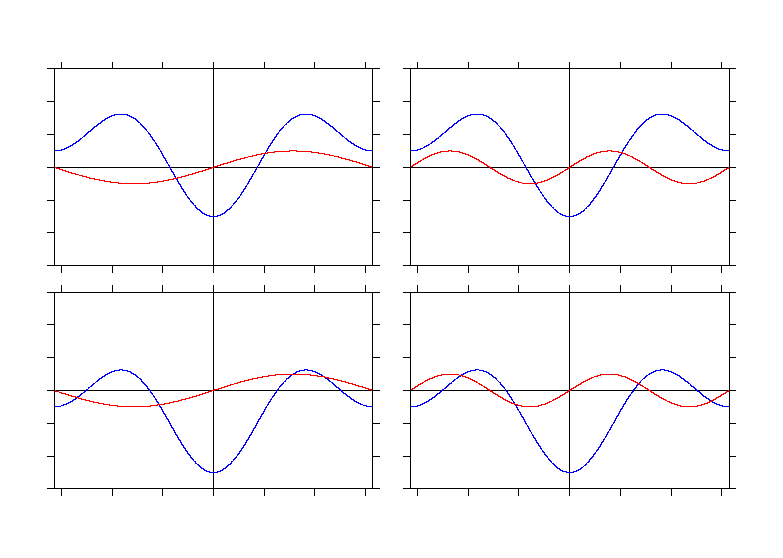
\includegraphics{Figures/Lattice.singlewire/dispersion/kdepend}}%
    \gplfronttext
  \end{picture}%
\endgroup
  
\caption{The numerically calculated gap $\Delta_k$ is plotted as a function of $k$ for different temperatures. Parameters: $k_F a_B = k_F a_{BF} = 0.3, l_t = 0, \frac{m_B}{m_F} = 0.8, \frac{n_B}{n_F^3} = 1$. }  
\label{fig.Deltakkdepend}  
\end{center}    
\end{figure}

\begin{figure} 
\begin{center}  
\input{Figures/Delta/Tdepend.tex}  
\caption{In black: The numerically calculated maximal pairing $\max_k[\Delta_k]$. In red: the asymptotic form from equation \eqref{eq.maxpairingasymp}. This is seen to fit very well for both $T/T_C \ll 1$ and $T/T_C \approx 1$. Notice, that the critical temperature at which the pairing vanishes is $T_C \approx 0.150 T_{F,0}$, and that the gap is rapidly decreasing in the region $0.10< T/T_{F,0} < 0.15$. Parameters: $k_F a_B = k_F a_{BF} = 0.3, l_t = 0, \frac{m_B}{m_F} = 0.8, \frac{n_B}{n_F^3} = 1$. }  
\label{fig.maxkDeltakTdepend}  
\end{center}    
\end{figure}

\begin{figure} 
\begin{center}  
\input{Figures/Delta/chempot.tex}  
\caption{In black: The numerically calculated chemical potential. Notice, that around the critical temperature, $T_C \approx 0.150 T_{F,0}$, the chemical potential jumps. In red: The free gas chemical potential. Parameters: $k_F a_B = k_F a_{BF} = 0.3, l_t = 0, \frac{m_B}{m_F} = 0.8, \frac{n_B}{n_F^3} = 1$. }  
\label{fig.chempot}  
\end{center}    
\end{figure}

 We observe for the solution at hand, that the pairing potential is uneven in $k$ as already argued, and that it goes to 0 for $k/k_F \gg 1$. This decay does not seem to be exponential, but rather of a power type. Further, the maximum value of the gap $\max_k[\Delta_k]$ decreases monotonically to 0 in a similar manner to the original BCS-theory. See \cite{Tinkham,BruusFlensberg,PlischkeStatPhys} for details. Finally, the chemical potential is plotted in figure \ref{fig.chempot}. Overall the (actual) numerically calculated chemical potential is lower and quite constant for $T/T_C \ll 1$. Then it starts rapidly increasing, compared to the free gas potential, and finally at $T_C$ it jumps to the free gas chemical potential. Physically, it is reasonable, that it starts out lower, since it should cost less energy to add another fermion, when they are (partially) attracting each other through the induced interaction. Further, the jump is inforced by the maximal gap going to $0$ at $T_C$. This can explicitly seen to be the case from \eqref{eq.HFFdef}, since the fermion Hamiltonian $H_{FF}$ goes to the \textit{free} fermion Hamiltonian, when $\Delta_k \to 0$. 

 We can enhance the pairing potential by decreasing the BEC scattering length $a_B$. This is connected to increasing the healing length $\tilde{\xi} = k_F\xi = \frac{\pi}{\sqrt{8 n_B/n_F^3 k_Fa_B}}$. In turn this is the range of the induced interaction in real space: $\tilde{V}_{FF}^\text{ind}(x,0) \propto \frac{\text{e}^{-|x|/2\xi}}{|x|}$. The enhancement is thus physically reasonable. This behaviour is seen to match with the depicted in figure \ref{fig.maxkDeltakaBdepend}, and it shows, that there is a dramatic increase for $k_Fa_B \to +0$, or equivalently when the range $\xi$ of the induced interaction goes to infinity. Further, the pairing actually crosses the free gas Fermi energy. In the same analysis we find, that the Fermi energy $\epsilon_F$ is shifted about $6\%$ from the free gas Fermi energy $\epsilon_{F,0}$ for all values of $k_F a_B$.  

\begin{figure} 
\begin{center}  
\input{Figures/DeltavaryaB/aBdepend.tex}  
\caption{The maximal pairing $\max_k[\Delta_k(T=0)]$ is plotted as a function of the BEC scattering length $a_B$. Notice that it increases dramatically for $k_Fa_B \to +0$ and actually exceeds the free gas Fermi energy in this limit. Other parameters: $k_F a_{BF} = 0.3, l_t = 0, \frac{m_B}{m_F} = 0.8, \frac{n_B}{n_F^3} = 1$.}  
\label{fig.maxkDeltakaBdepend}  
\end{center}    
\end{figure}


 We now turn our attention to the potential width for the string: $l_t$. Finding a solution for $l_t > 0$ is a little more tedious than for $l_t = 0$, since we then need to solve the integral for $V_{FF}^\text{ind}(q,0)$ for each iteration. It does however carry through analogously to the $l_t = 0$ case. Figure \ref{fig.maxkDeltakltdepend} shows the found dependency on $l_t$ of the maximal pairing. We see, that there is a well defined $l_t \to 0$ limit as expected, and that the maximal pairing decreases monotonically with $l_t$. This can best be understood again from the real space induced interaction. We saw in figure \ref{fig.Vx}, that the induced interaction is effectively shielded around $x = 0$ for $l_t > 0$. This shielding is increased for higher values of $l_t$. Hence, the interaction is lowered when the particles are close to each other. In conclusion the pairing most decrease with increasing $l_t$. 

\begin{figure} 
\begin{center}  
\input{Figures/Deltavarylt/ltdepend.tex}  
\caption{The maximal pairing $\max_k[\Delta_k(T=0)]$ is plotted as a function of the potential width $l_t$. Other parameters: $k_Fa_B = k_F a_{BF} = 0.3, \frac{m_B}{m_F} = 0.8, \frac{n_B}{n_F^3} = 1$.}  
\label{fig.maxkDeltakltdepend}  
\end{center}    
\end{figure}

Let us now investigate the dependency on the fermion-boson scattering length: $a_{BF}$. The result of the numerical calculation is shown in \ref{fig.maxkDeltakaBFdepend}. The pairing is seen to drop to zero around $k_Fa_{BF,c} = 0.155$. This shows, that the fermion-boson scattering length must exceed a cricital value for the string to be superconducting.   

\begin{figure} 
\begin{center}  
\input{Figures/DeltavaryaBF/aBFdepend.tex}  
\caption{The maximal pairing $\max_k[\Delta_k(T=0)]$ is plotted as a function of the fermion-boson scattering length $a_{BF}$. Notice that it goes rapidly to zero around $k_Fa_{BF} = 0.155$. Other parameters: $k_F a_{B} = 0.001, l_t = 0, \frac{m_B}{m_F} = 0.8, \frac{n_B}{n_F^3} = 1$.}  
\label{fig.maxkDeltakaBFdepend}  
\end{center}    
\end{figure}

